Classic question on transient behaviour of a laser.

\begin{parts}
	\part Relaxation oscillation: variation in laser output as a result of disturbance to the system, e.g. change in cavity length, this is more regularly spaced and gentler than laser spiking.
	
	Laser spiking: sharp and rather irregular spikes in laser output when it is first turned on.
	
	The reason why both conditions occur is due to the underdamp in the cavity mode and may be summarised as $\tau_2 \ll \tau_c$ where $\tau_2$ is the lifetime of the upper level, $\tau_c$ is the cavity lifetime.
	
	\part $N^*_s$: threshold population inversion -- this is the boundary of population inversion beyond which photon population begins to grow.
	
	\begin{figure}[H]
		\centering
		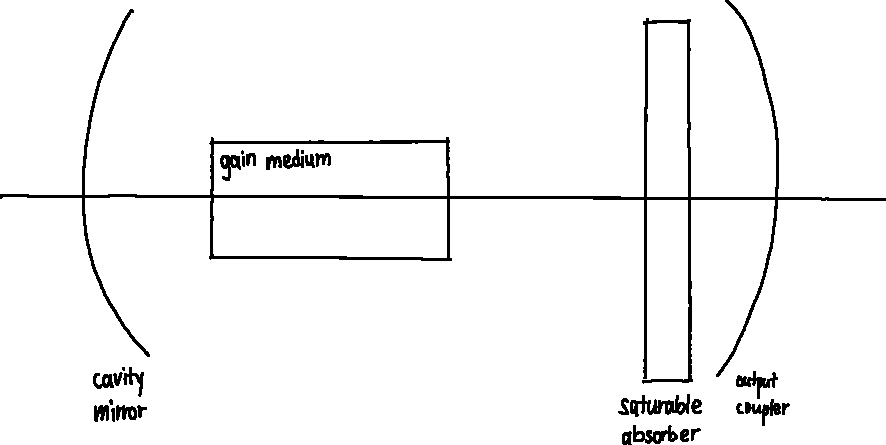
\includegraphics[width=.7\linewidth]{q1-cavity}
	\end{figure}
	
	In the absence of gain, we have:
	\begin{align*}
		\deri{n}{t} &= -\underbracket{\rbracket{\frac{1}{2}nc}}_{\textnormal{flux in each direction}} \cdot \underbracket{A_\textnormal{cavity}}_{\textnormal{beam cross-sectional area}} \cdot \frac{\rbracket{1-R_1} + \rbracket{1-R_2}}{\underbracket{V_\textnormal{cavity}}_\textnormal{cavity volume}} \\
		&= -\frac{1}{2}nc \cdot \frac{1}{L} \cdot \rbracket{0 + T} \\
		&= -\frac{cT}{2L}n \equiv -\frac{n}{\tau_c} \\
		\Rightarrow \tau_c &= \frac{2L}{cT}
	\end{align*}
	
	Cavity round-trip time is given as:
	\begin{equation*}
		t_\textnormal{rt} = \frac{2L}{c} \Rightarrow \tau_c = t_\textnormal{rt}/T
	\end{equation*}
	
	At steady state, $\dderi{N^*}{t} = \dderi{n}{t} = 0$:
	\begin{align*}
		\frac{1}{\eta} \frac{N^*}{N^*_s} \frac{n}{\tau_c} + \frac{N^*}{\tau_2} &= S_2 \\
		\xRightarrow{N^*/N^*_s - 1 = 0 \Rightarrow N^* = N^*_s} \frac{1}{\eta} \cdot \frac{n}{\tau_c} &= S_2 - \frac{N_s^*}{\tau_2} \\
		\Rightarrow n_{ss} &= \eta\tau_c \sbracket{S_2 - \frac{N_s^*}{\tau_s}}
	\end{align*}
	
	In the absence of stimulated emission:
	\begin{align*}
		\deri{N^*}{t} &= S_2 - \frac{N^*}{\tau_2} \\
		\Rightarrow N^*(0) &= S_2 \tau_2 \mtext{at steady state}
	\end{align*}
	
	Hence overpumping ratio $r = \dfrac{S_2 \tau_2}{N^*_s} = \dfrac{N^*(0)}{N^*_s}$.
	
	\part For small perturbation we have:
	\begin{align*}
		N^* &= N^*_\textnormal{ss} + \Delta N^* \\
		n &= n_\textnormal{ss} + \Delta n_{ss}
	\end{align*}
	where $X_\textnormal{ss}$ is steady state value of $X$.
	
	Plugging them into the rate equations gives:
	\begin{align*}
		\deri{N^*}{t} &= \deri{(\Delta N^*)}{t} \\
		&= S_2 - \frac{1}{\eta} \frac{\rbracket{N^*_s + \Delta N^*}}{N^*_s} \cdot \frac{\rbracket{n_\textnormal{ss} + \Delta n}}{\tau_c} - \frac{N^*_s + \Delta N^*}{\tau_2} \\
		&= S_2 - \frac{1}{\eta\tau_c} \rbracket{1 + \frac{\Delta N^*}{N^*_s}} \rbracket{n_\textnormal{ss} + \Delta n} - \frac{N^*_s + \Delta N^*}{\tau_2} \\
		&\simeq S_2 - \frac{1}{\eta\tau_c} \rbracket{n_\textnormal{ss} + \Delta n + \frac{n_\textnormal{ss}}{N^*_s} \Delta N^*} - \frac{N^*_s + \Delta N^*}{\tau_2} \textnormal{\hspace{.5em}keeping 1st order terms} \\
		&= S_2 - S_2 + \frac{N^*_s}{\tau_2} - \frac{\Delta n}{\eta\tau_c} - \rbracket{S_2 - \frac{N^*_s}{\tau_2}} \cdot \frac{\Delta N^*}{N^*_s} - \frac{N^*_s}{\tau_2} - \frac{\Delta N^*}{\tau_2} \\
		&= -\Delta N^*\sbracket{\frac{S_2}{N^*_s}} - \frac{\Delta n}{\eta\tau_c} \\
		&= -\frac{r}{\tau_2} \Delta N^* - \frac{\Delta n}{\eta\tau_c}
	\end{align*}
	
	\begin{align*}
		\deri{n}{t} = \deri{(\Delta n)}{t} &= \underbracket{\sbracket{\frac{N^*_s + \Delta N^*}{N^*_s} - 1}}_{\Delta N^*} \frac{n_\textnormal{ss} + \Delta n}{\tau_c} \\
		&\simeq \frac{n_\textnormal{ss}}{\tau_c} \frac{\Delta N^*}{N^*_s} \mtext{by linearisation} \\
		&= \eta \rbracket{S_2 - \frac{N^*_s}{\tau_2}} \Delta N^* \\
		&= \frac{\eta}{\tau_2} \underbracket{\rbracket{\frac{S_2 \tau_2 - N^*_s}{N^*_s}}}_{r-1} \Delta N^*
	\end{align*}
	
	Now insert ansatz $\Delta N^* = a\mathrm{e}^{mt}$, $\Delta n = b\mathrm{e}^{mt}$:
	\begin{align*}
		\deri{n}{t} &= bm\mathrm{e}^{mt} = \frac{(r-1) \eta}{\tau_2} a\mathrm{e}^{mt} \\
		\Rightarrow m &= \frac{(r-1) \eta}{\tau_2} \frac{a}{b} \Rightarrow \frac{b}{a} = \frac{(r-1) \eta}{\tau_2 m} \\[.5em]
		%
		\deri{\Delta N^*}{t} &= -\frac{r}{\tau_2} a\mathrm{e}^{mt} - \frac{1}{\eta \tau_c} b\mathrm{e}^{mt} \\
		\Rightarrow m &= -\frac{r}{\tau_2} - \frac{1}{\eta \tau_c} \frac{b}{a}
	\end{align*}
	
	Hence:
	\begin{gather*}
		m + \frac{1}{\eta \tau_c} \cdot \frac{(r-1) \eta}{\tau_2 m} = -\frac{r}{\tau_2} \\
		\Rightarrow m^2 + \frac{r}{\tau_2} m + \frac{r-1}{\tau_c \tau_2} = 0 \\
		m = \frac{-r/\tau_2 \pm \sqrt{(r/\tau_2)^2 - 4(r-1)/\tau_c \tau_2}}{2}
	\end{gather*}
	
	We want $m$ to be complex for oscillations:
	\begin{align*}
		\rbracket{\frac{r}{\tau_2}}^2 - \frac{4(r-1)}{\tau_c \tau_2} &< 0 \\
		\frac{r^2}{\tau_2} &< \frac{4(r-1)}{\tau_c}
	\end{align*}
	Note that the scenario $\tau_2 \ll \tau_c$ satisfies this inequality.
	
	Thus we have the angular frequency ($\omega_{ro}$) and frequency ($f_{ro}$) of relaxation oscillations:
	\begin{align*}
		\omega_{ro}^2 &= \frac{1}{4} \sbracket{\frac{4(r-1)}{\tau_2 \tau_c} - \rbracket{\frac{r}{\tau_2}}^2} \\
		f_{ro} &= \frac{\omega_{ro}}{2\pi}
	\end{align*}
	
	In the limit $\tau_2 \ll \tau_c$, $\omega_{ro}^2 \rightarrow (r-1)/\tau_2 \tau_c$, so:
	\begin{align*}
		r-1 &= \rbracket{2\pi f_{ro}}^2 \tau_2 \tau_c \\
		r &= \rbracket{2\pi f_{ro}}^2 \tau_2 \tau_c + 1 \\
		\frac{N^*(0)}{N^*_s} &= \rbracket{2\pi f_{ro}}^2 \frac{\tau_2 t_\textnormal{rt}}{T} + 1 \\
		\eta N^*(0) \sigma_{21} \underbracket{c \tau_c}_{2L/T} &= \ldots \\
		\Rightarrow \delta &= \rbracket{2\pi f_{ro}}^2 \tau_2 t_\textnormal{rt} + T
	\end{align*}
	
	\part From above, we have $f_{ro} \propto \sqrt{r} \propto \sqrt{S_2}$ the pump rate, hence the graph exhibits a square root dependency.
	
	In addition, as the oscillations in laser power are of frequency $f_{ro}$, the frequency spectrum should exhibit a peak at $f_{ro}$.
	
	From the graph, we infer that $f_{ro} \simeq \SI{190}{\kilo\hertz}$ @ $\SI{1000}{\milli\watt}$ pump power.
	
	With $t_\textnormal{rt} = \SI{4}{\nano\second}$, $\tau_2 = \SI{450}{\micro\second}$, $T = 9.5\%$, we have $\delta = 2.660$.
	
	The advantage of this method is that the measurement error in cavity dimensions do not get into the calculation, enhancing the accuracy of gain measurement.
\end{parts}